\section{Scalar field on Schwarzschild space-time}
Although the final goal in this field is to compute tensor waveforms that can be used as templates for LISA searches, for the purposes of obtaining the desired accuracy, it is important to improve our computational methods. We do this by developing numerical techniques using scalar, rather than tensor, self force methods to make the problem more tractable. I have reimplemented Peter Diener's Fortran scalar self-force code, with a slightly modified design, in C++. The desired goal was for the results to match to within roundoff error. This was achieved for scalar fields without a source and for scalar fields with point sources on circular orbits (see Chapter~\ref{circularorbit}). The original goal, currently put on hold, was to parallelize this code in HPX, a tool which makes it simple to do high performance computing. In this chapter, I discuss the physical behavior of a scalar field without a source on a Schwarzschild background. 


\subsection{Scalar field wave equations}
A scalar field is a field that has one one degree of freedom at a given point in space-- rather than being a matrix, it has a single value. The scalar wave equation can be written, in the absence of a source, in short form, as the D'Alembertian or box operator acting on a scalar field. 
\begin{equation}
  \Box\Psi=0
\end{equation}
In flat spacetime this reduces to the standard wave equation. In curved spacetime, further complications are introduced, to account for the curvature of space. This enters through the metric. For a scalar field, the D'Alembertian can be written
\begin{equation}
  \Box\Psi=\frac{1}{\sqrt{-g}}\partial_\mu(\sqrt{-g}g^{\mu\nu}\partial_\nu\Psi)=0
\end{equation}
where $g$ is the determinant of $g_{\mu\nu}$.~\cite{Wald} 

\subsubsection{Multipole moment decomposition}

In our approach, spherical harmonics are used to reduce the three spatial dimensions to a one dimensional problem, in terms of the radius and a sum of an infinite number of discrete spherical harmonic modes, characterized by numbers $l$ and $m$, where $l$ ranges from $0$ to $\infty$ and  $m$ ranges from $-l$ to $+l$ for each $l$~\cite{poisson_pound_vega_living_review}. The field is written as
\begin{equation}
  \Psi=\sum_{l,m}\Psi^{lm}(t,r)Y^{lm}(\theta,\phi)
\end{equation}
This separation of variables ansatz can be used to simplify the wave equation in any coordinate system, since the angular coordinates are not transformed in any of the coordinate systems we use. We make use of the identity
\begin{equation}
  r^2\nabla_{\theta,\phi}^2Y^{lm}=-l(l+1)Y^{lm}
\end{equation}
where $\nabla_{\theta,\phi}^2$ is the angular part of the Laplacian, which has a $\frac{1}{r^2}$ dependence. This introduces a term proportional to $l(l+1)\Psi^{lm}(t,r)$ for each $l$, $m$. 

\subsubsection{Tortoise coordinates}
In this code, we use a mixture of tortoise (Eddington-Finkelstein) and hyperboloidal coordinates. Tortoise coordinates have the property that they go to infinity at the horizon and spatial infinity. It is beneficial to place the horizon at an unreachable distance in coordinate space so that the boundary conditions at the horizon become trivial and there is no leakage of information from the interior of the black hole to outside the horizon in the process of discretization. It is also beneficial to increase the number of computational elements near the horizon by compactifying the coordinates there. Tortoise coordinates are obtained by the following transformation of Schwarzschild coordinates.~\cite{Wald}
\begin{eqnarray}
  t_*=t\\
  r_*=r+2M\ln|\frac{r}{2M}-1|\\
  \theta_*=\theta\\
  \phi_*=\phi
\end{eqnarray}
We solve the wave equation in tortoise coordinates in one region of the code. I have re-derived this equation in Mathematica and verified the form that appears in Peter Diener's Fortran scalar self-force code. The wave equation in tortoise coordinates is
\begin{equation}
  \frac{\partial^2\psi}{\partial t^2}=\frac{\partial^2\psi}{\partial r_*^2}-\frac{1}{r^3}\left(\frac{2M}{r}+(l+1)l\right)\left(1-\frac{2M}{r}\right)\psi
\end{equation}
$r$ is in Schwarzschild coordinates, $r_*$ is in tortoise coordinates, $l$ is the spherical harmonic l-mode (discussed below), which accounts for the angular dependence, and $\psi$ is a function of tortoise coordinates.


\subsubsection{Hyperboloidal coordinates}  
Hyperboloidal coordinates are necessary because infinities are computationally unreachable. It is clear that space infinitesimally close to the horizon is important, since the curvature of space is strongest there, and it is still causally connected to the exterior region. To make the horizon reachable in a finite number of computational elements, while retaining the property that more computational elements are placed near the horizon than far away, hyperboloidal coordinates are introduced in the region closest to the horizon. In a middle region, tortoise coordinates are used. In the region furthest from the black hole, hyperboloidal coordinates are used again to place light-like infinity, $\mathcal{I}^+$, at a finite coordinate. 



There are a few key features of the hyperboloidal transformation~\cite{bernuzzi_nagar_zenginoglu_hyperb}. The angular coordinates are not transformed. The time coordinate preserves the stationarity of the background metric, and thus the new time variable, $\tau$, must be related to the old time variable, $t_*$, by an offset dependent only upon $r_*$, $\tau=t-h(r_*)$. For in-going waves in the inner region, $t-r_*=\tau+\rho$ and in the outgoing region, $t+r_*=\tau-\rho$ to preserve the structure of the light cone. Bernuzzi, Nagar, and Zenginoglu define $H=\frac{dh}{dr_*}$. They introduce a compactification that depends on a transition function $\Omega$~\cite{OmegaTransferFunction} that goes to one at the horizon, is constant in the tortoise region, and smoothly goes to zero in the outer hyperboloidal region. The tortoise coordinate is defined to be  $r_*=\frac{\rho}{\Omega(\rho)}$ in the hyperboloidal region, resulting in an expression for the height function $H$ in terms of the hyperboloidal radius,  $H(\rho)=1-\frac{\Omega^2}{\Omega-\rho\Omega^\prime}$. For the purpose of computing characteristic modes, important for the numerical fluxes, we are only interested in the highest derivative terms of the wave equation, called the principal part. Their final principle part of the wave equation, for in-going waves, is~\cite{bernuzzi_nagar_zenginoglu_hyperb}
  \begin{eqnarray}
    \partial_{t_*}^2-\partial_{r_*}^2=&-(1-H^2)\partial_\tau^2\nonumber\\
    &+(1-H)(-2H\partial_\tau\partial_\rho+(1-H)\partial_\rho^2-(\partial_\rho H)(\partial_\tau+\partial_\rho))
  \end{eqnarray}    
I have verified this equation, and derived the out-going wave equation, in Mathematica.

  



\section{Theoretical expectations}

The system without a source is necessary for code development; however, it is also similar to the like the ring-down phase of an EMRI system after the small black hole plunges into the super-massive black hole. There are two analytically predicted behaviors that characterize the system that has no source. Initially,there should be quasi-normal mode ringing. Eventually that fades into a long, power law tail. 

\subsection{Quasi-normal modes}
A field, such as a scalar or tensor field surrounding a black-hole, exhibits quasi-normal mode ringing as it relaxes into or away from the black hole.  
In EMRI's, quasi-normal modes are expected to be detected by LISA after the small black hole crosses the large black hole's horizon, following the plunge from the innermost stable circular orbit. In LIGO, the fundamental quasi-normal mode was seen after the merger phase during the ring-down phase in LIGO's first detection~\cite{LIGO1e}. The same set of quasi-normal modes is expected for any tensor field perturbed around a black hole, regardless of why, as long as there is no source present. The case is very similar with scalar fields, though the spectrum and decay rates of quasi-normal modes is slightly different.

A quasi-normal mode decays at a steady frequency with an exponential decay envelope due to loss of energy from the system. These rates have been calculated by Reference~\cite{bertiSchwQNM} and made available online. I have tested their theoretical expectations for the fundamental mode at each l-mode against my simulation data in Figures~\ref{qnml1m1} and~\ref{qnml2m2} by plotting the QNM ringdown waveform using Berti's frequency and exponential decay parameters and adjusting the amplitudes and starting times by hand. Notice that for higher $l$, the quasi-normal mode frequency is higher and the decay is faster.

\begin{figure}
  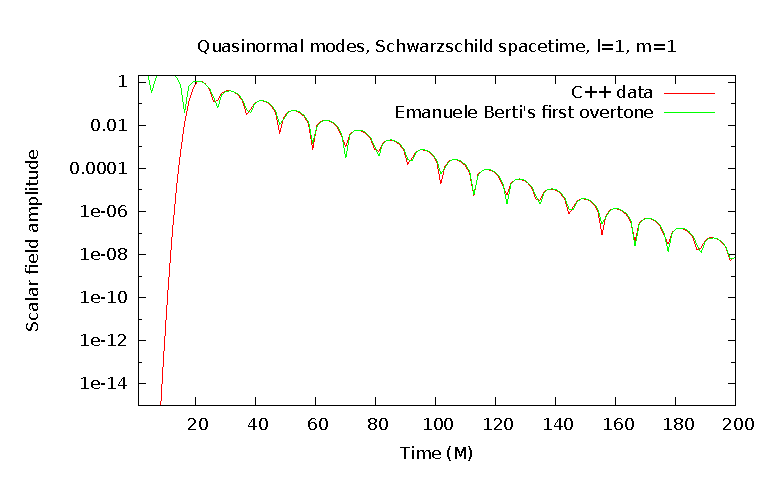
\includegraphics{l1m1qnm}
  \caption{Fundamental quasi-normal mode for l=1}
  \label{qnml1m1}
\end{figure}

\begin{figure}
  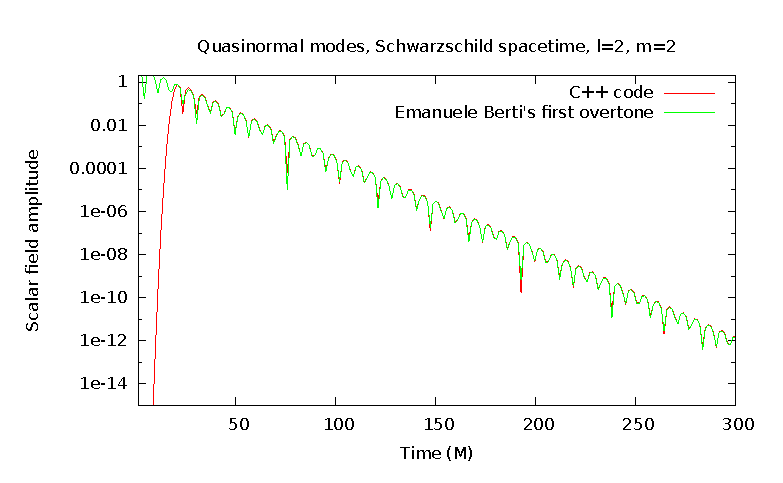
\includegraphics{l2m2qnm}
  \caption{Fundamental quasi-normal mode for l=2}
  \label{qnml2m2}
\end{figure}


\subsection{Power law tails}

Quasi-normal mode ringing evolves into power law tails with a relatively rapid transition between the two regimes. Both are due to backscattering of the waves off the background metric, but for EMRI's, QNM are due to interactions near the horizon of the supermassive black hole (post-merger) while the power law tails are due to interactions of the field with the background spacetime far away from it. In 1972, Richard Price predicted that the tails would scale as $t^{-(2l+2)}$ or $t^{-(2l+3)}$ depending on initial conditions~\cite{PriceTails}. In our choice of initial conditions, $t^{-(2l+3)}$ matches best for the choices of $l$ explored. Figure~\ref{taill1m1} shows a mode for which I successfully recovered a power law tail. Figure~\ref{notaill2m2} demonstrates that truncation error may dominate at high l, and that it may be necessary to increase the DG order to resolve all l-modes in a simulation.

\begin{figure}
  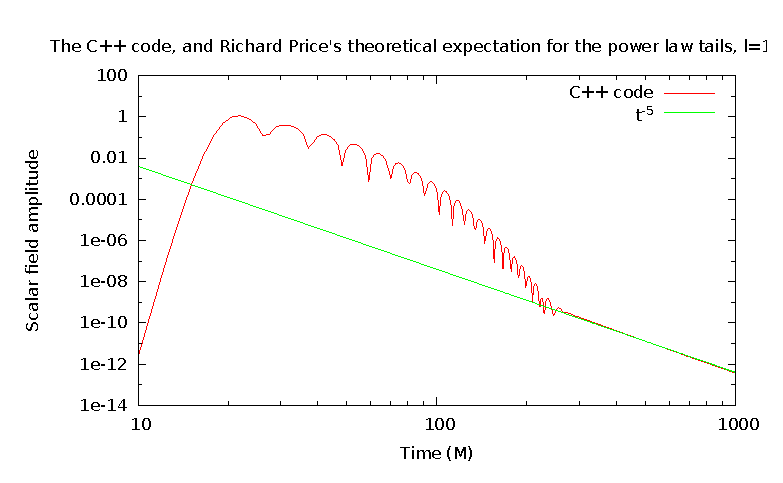
\includegraphics{l1m1tail2}
  \caption{Power law tail, l=1}
  \label{taill1m1}
\end{figure}

\begin{figure}
  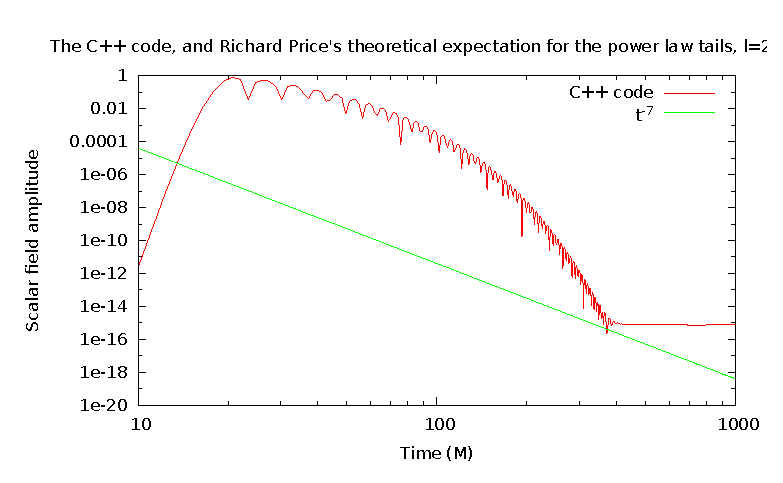
\includegraphics{l2m2tailfail2}
  \caption{Power law tail does not match expectations due to truncation error in DG method, l=2}
  \label{notaill2m2}
\end{figure}

